% !TEX program = pdflatex
% Manuscript target: Classical and Quantum Gravity (IOP Publishing)
% Official IOP submission class (local iopjournal.cls, 2024+)
% Signature convention: (-,+,+,+); geometric units c = G = 1
\documentclass{iopjournal}

\usepackage{amsmath,amssymb,amsfonts,amsthm}
\usepackage{microtype}
% graphicx and hyperref are loaded by iopjournal.cls

% iopart-compatible front-matter aliases (map onto iopjournal natives)
\newcommand{\address}{\affil}
\newcommand{\ead}{\email}

\newcommand{\Phir}{\Phi(r)}
\newcommand{\br}{b(r)}
\newcommand{\omegar}{\omega(r)}
\newcommand{\Gmn}{G_{\mu\nu}}
\newcommand{\Tmn}{T_{\mu\nu}}
\newcommand{\Rmn}{R_{\mu\nu}}
\newcommand{\Mcal}{\mathcal{M}}
\newcommand{\MN}{\mathcal{M}_{N}}
\newcommand{\phif}{\varphi_{\mathrm{st}}}

\newtheorem{theorem}{Theorem}[section]
\newtheorem{proposition}[theorem]{Proposition}
\newtheorem{lemma}[theorem]{Lemma}
\newtheorem{definition}[theorem]{Definition}
\theoremstyle{remark}
\newtheorem{remark}[theorem]{Remark}

\begin{document}

\articletype{Paper}

\title{Discrete Spacelike Monodromy Proxy and Infrared Spectral Transition on Axisymmetric Frame-Dragging Backgrounds}

\author{Mauricio Miguel Paniagua Ramirez$^{1,2}$}

\address{$^{1}$Faculty of Electrical Engineering, Universidad Michoacana de San Nicol\'as de Hidalgo (UMSNH), Morelia, Michoac\'an, Mexico}

\address{$^{2}$Faculty of Mathematics and Computer Science, FernUniversit\"at in Hagen, Hagen, Germany}

\ead{1912574a@umich.mx}

\ead{mauricio.paniagua@studium.fernuni-hagen.de}

\keywords{general relativity, wormholes, frame dragging, ergoregion, discrete monodromy, spectral radius, mass gap}

\begin{abstract}
We analyze the spectral structure of a discrete azimuthal transport proxy on stationary, axisymmetric Morris--Thorne geometries with frame dragging.
Closed-form metric profiles $\{b(r),\Phi(r),\omega(r)\}$ define a Lorentzian background with flare-out at the throat and an equatorial ergoregion (bounded by the ergosurface $\Sigma_{\mathrm{ERGO}}$) wherever $e^{2\Phi(r)}<r^{2}\omega(r)^{2}$, equivalently $g_{tt}>0$ [criterion~(C1)].
A retarded kernel with mode-augmented mass $m_{\ast}$ is sampled on an $N$-node spacelike azimuthal circle at fixed $(r,\theta)$---where $g_{\varphi\varphi}>0$---as a \emph{discrete spacelike monodromy proxy}; the row-sum renormalized gate is contractive by construction, while the \emph{unnormalized} discrete proxy $\widetilde{K}$ provides the infrared spectral diagnostic [criterion~(C3)].
The row-sum renormalized matrix $K$ is a numerical control gate with $\rho(K)<1$ by algebraic design; the infrared diagnostic is carried by the unnormalized proxy $\widetilde{K}$, for which we identify a mass-gap threshold: at azimuthal mode $\nu=0$ the exponential massless proxy satisfies $\rho(\widetilde{K}_{N})\to 2\pi\sqrt{g_{\varphi\varphi}}\simeq 9.42>1$ as $m^{2}\to 0$, so discrete-proxy contractivity fails in the massless infrared on this spacelike wormhole loop.
High-resolution spectral diagnostics corroborate both the control-gate behaviour and the discrete-proxy spectral rupture up to $N=1024$.
The equatorial Einstein tensor is obtained by symbolic differentiation as a static background constraint [criterion~(C2)].
No continuum closed-timelike-curve field theorem, and no Hadamard-state or renormalized-stress-energy theorem, are claimed.
\end{abstract}

\section{Introduction}
\label{sec:intro}

Stationary axisymmetric geometries with frame dragging provide controlled Lorentzian backgrounds on which one can test discrete transport operators and their spectral radii without evolving the Einstein equations~\cite{Morris1988,Visser1995}.
Questions of field self-consistency on chronologically nontrivial spacetimes have a long history~\cite{Hawking1992,Novikov1989,Friedman1990,KimThorne1991}, but the object analyzed here is narrower and purely spectral: a finite-dimensional monodromy matrix assembled by sampling a retarded kernel on a coordinate azimuthal circle.
That circle is spacelike ($g_{\varphi\varphi}>0$); the construction is therefore a \emph{spacelike} loop-transport proxy on a fixed stationary wormhole background, not a continuum theorem about closed timelike curves.

\paragraph{Scope and non-claims.}
The numerical analysis evaluates exclusively a discrete monodromy proxy sampled on a coordinate azimuthal loop at fixed $(r,\theta)$: spectral radii, contraction diagnostics, and Picard fixed points for the matrices $K$ and $\widetilde{K}$ of Sec.~\ref{sec:monodromy}.
It does \emph{not} solve a fully dynamical Klein--Gordon field coupled to the gravitational background in real time, nor does it evolve the Einstein equations or reconstruct a continuum Green function on~\eqref{eq:metric}.
It likewise does \emph{not} establish existence of closed timelike curves in~\eqref{eq:metric}, nor prove continuum field self-consistency theorems on causal closed curves.
Semiclassical Hadamard renormalization, Kay--Radzikowski--Wald-type no-go statements, and curvature-cutoff models of $\langle\Tmn\rangle_{\mathrm{ren}}$ lie outside the certified scope of this work.

We organize the contribution around three criteria of decreasing computational status:
\begin{enumerate}
  \item[(C1)] \textbf{Geometric regularity:}
    smooth profiles with flare-out and an equatorial ergoregion $e^{2\Phir}<r^{2}\omegar^{2}$ (where $g_{tt}>0$ and $\partial_{t}$ is spacelike), bounded by the ergosurface $\Sigma_{\mathrm{ERGO}}$;
  \item[(C2)] \textbf{Symbolic background stress-energy:}
    equatorial $\Gmn$ and NEC/WEC contractions obtained by symbolic differentiation as static constraints, not as dynamically evolved curvature tensors;
  \item[(C3)] \textbf{Discrete Sobolev contraction and mass-gap threshold (core result):}
    unique fixed point of the row-sum--renormalized gate in the massive regime, together with a spectral rupture $\rho(\widetilde{K})\to 2\pi\sqrt{g_{\varphi\varphi}}>1$ as $m^{2}\to 0$ at $\nu=0$ for the unnormalized spacelike proxy.
\end{enumerate}

Throughout, ``continuous'' statements motivate the kernel form; all certified numerical claims refer to the discrete operator $\MN$ constructed in Sec.~\ref{sec:monodromy}.
Criterion~(C3)---the infrared spectral transition of the unnormalized proxy---is the primary result.

%==============================================================================
\section{Geometry and profile class}
\label{sec:geometry}

We adopt a stationary, axisymmetric Morris--Thorne line element with azimuthal frame dragging,
\begin{equation}
\label{eq:metric}
\begin{split}
\mathrm{d}s^{2}
&= -e^{2\Phir}\,\mathrm{d}t^{2}
 + \frac{\mathrm{d}r^{2}}{1-\br/r}
 + r^{2}\,\mathrm{d}\theta^{2} \\
&\quad + r^{2}\sin^{2}\theta\,\bigl(\mathrm{d}\varphi - \omegar\,\mathrm{d}t\bigr)^{2},
\end{split}
\end{equation}
in the same geometric class as rotating traversable wormhole metrics with an ergoregion~\cite{Morris1988,Visser1995,Teo1998}.
Coordinates are $x^{\mu}=(t,r,\theta,\varphi)$ and
$\det(g_{\mu\nu})=-r^{5}e^{2\Phir}\sin^{2}\theta/(r-\br)$.

\subsection{Explicit metric profiles}

We specify the closed-form parameterization used throughout the numerical and symbolic analyses,
\begin{align}
\label{eq:profiles}
\br &= r_{0}\Bigl(\frac{r_{0}}{r}\Bigr)^{\gamma},
& \Phir &= -\frac{\alpha r_{0}}{r},
& \omegar &= \omega_{0}\exp\!\Bigl[-\beta\frac{r-r_{0}}{r_{0}}\Bigr],
\end{align}
with $\gamma>0$, $\alpha\ge 0$, $\omega_{0}>0$, and $\beta>0$.
At the throat $r=r_{0}$: $b(r_{0})=r_{0}$ and $b'(r_{0})=-\gamma$, so the flare-out condition $b'<1$ holds whenever $\gamma>0$~\cite{Morris1988}.

\paragraph{Reference parameters.}
Unless otherwise stated, numerical diagnostics use the reference profile
\begin{equation}
\label{eq:ref-params}
r_{0}=1,\quad
\gamma=0.5,\quad
\alpha=0.1,\quad
\omega_{0}=1.2,\quad
\beta=2.0,
\end{equation}
with the discrete monodromy proxy and the supporting geodesic diagnostic assembled at the sampling radius $r_{\mathrm{loop}}=1.5\,r_{0}$.
The symbol $r_{\mathrm{loop}}$ labels a fixed-coordinate radius for that sampling circle; it does \emph{not} designate a closed causal curve.

\paragraph{Admissibility bounds (C1).}
\begin{align}
\label{eq:bounds}
\gamma &> 0
&& \text{(flare-out)}, \nonumber\\
e^{-2\alpha} &< r_{0}^{2}\omega_{0}^{2}
&& \text{(ergoregion opens at throat)}, \nonumber\\
r_{\mathrm{ERGO}} &> r_{0}
&& \text{(ergosurface exterior to throat)}.
\end{align}
The geometric boundary analyzed below is the equatorial ergosurface $\Sigma_{\mathrm{ERGO}}$: its radius $r_{\mathrm{ERGO}}$ is the smallest $r>r_{0}$ solving $e^{2\Phir}=r^{2}\omegar^{2}$ (equivalently $g_{tt}=0$ at $\theta=\pi/2$), computed by bisection.

\subsection{Frame dragging, ergosurface, and ergoregion}

The stationary Killing norm
\begin{equation}
\label{eq:gtt}
g_{tt}=-e^{2\Phir}+r^{2}\sin^{2}\theta\,\omegar^{2}
\end{equation}
vanishes on the equatorial ergosurface
\begin{equation}
\label{eq:Sigma-ERGO}
\Sigma_{\mathrm{ERGO}}
:=\bigl\{x^{\mu}:\ \theta=\pi/2,\ \ g_{tt}(x)=0\bigr\}
=\bigl\{x^{\mu}:\ \theta=\pi/2,\ \ e^{2\Phir}=r^{2}\omegar^{2}\bigr\}.
\end{equation}
Wherever
\begin{equation}
\label{eq:ergo-open}
e^{2\Phir} < r^{2}\omegar^{2},
\end{equation}
one has $g_{tt}>0$, so $\partial_{t}$ is spacelike: that open set is the equatorial ergoregion, bounded by $\Sigma_{\mathrm{ERGO}}$.
We emphasise the ontological separation used throughout:
\begin{itemize}
  \item $\Sigma_{\mathrm{ERGO}}$ is an \emph{ergoregion boundary} defined by $g_{tt}=0$;~\eqref{eq:ergo-open} marks the failure of static stationarity for $\partial_{t}$-observers.
  \item Appearance of an ergoregion is \emph{not} the onset of closed timelike curves, nor a chronology horizon, nor a change in the topology of closed curves in the $\varphi$-direction.
\end{itemize}
In particular, the fixed-$(t,r,\theta)$ azimuthal circle used by the monodromy proxy has tangent $\partial_{\varphi}$ with
\begin{equation}
\label{eq:gphiphi}
g(\partial_{\varphi},\partial_{\varphi})
=
g_{\varphi\varphi}
=
r^{2}\sin^{2}\theta
>0
\end{equation}
in the signature $(-,+,+,+)$, and is therefore a \emph{spacelike} circle for every $r>r_{0}$ (including $r=r_{\mathrm{loop}}$).
Its proper arc-length element is written
\begin{equation}
\label{eq:Delta-ell}
\Delta\ell
=
\sqrt{g_{\varphi\varphi}}\,\Delta\varphi,
\end{equation}
and is \emph{not} a proper-time increment of a timelike worldline.
The co-rotating combination $\xi=\partial_{t}+\omegar\partial_{\varphi}$ satisfies $g(\xi,\xi)=-e^{2\Phir}<0$ and therefore remains timelike across $\Sigma_{\mathrm{ERGO}}$, but the integral curves of $\xi$ are not the sampling circle of the discrete proxy.
Null slopes in the $(t,\varphi)$ subspace are
\begin{equation}
\label{eq:null-slopes}
\Bigl(\frac{\mathrm{d}\varphi}{\mathrm{d}t}\Bigr)_{\!\pm}=\omegar\pm e^{\Phir}/r,
\end{equation}
so inside the ergoregion the future light cone encompasses $-\partial_{t}$ (Fig.~\ref{fig:lightcones}).

Christoffel symbols used for geodesic diagnostics are obtained from~\eqref{eq:metric} by central finite differences with step $\varepsilon=10^{-5}$.
As a supporting geometric check---distinct from the spacelike monodromy circle---we integrate the co-rotating timelike geodesic with initial tangent $u\propto(1,0,0,\omega)$ at $r=r_{\mathrm{loop}}$, so that $g(u,u)=-e^{2\Phir}<0$ (equivalently normalized to $g(u,u)=-1$), by classical RK4 with proper-time step $\Delta\tau=0.01$ along that timelike curve (Fig.~\ref{fig:geodesic}).
This geodesic diagnostic does not identify the sampling locus of Sec.~\ref{sec:monodromy} with a closed causal curve.

\begin{figure}[t]
\centering
\begin{minipage}{0.48\textwidth}
\centering
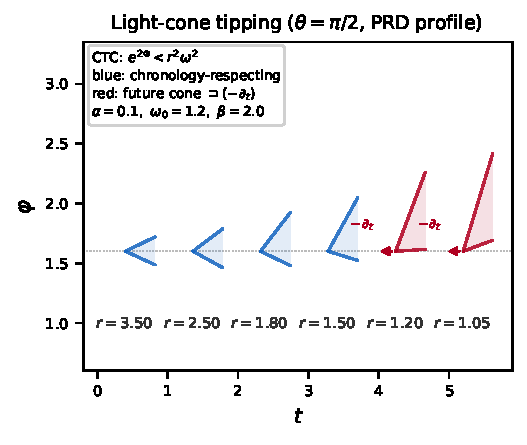
\includegraphics[width=\linewidth]{figures/lightcones.pdf}
\caption{Light-cone tipping in the equatorial $(t,\varphi)$ plane for the reference profiles~\eqref{eq:ref-params}. Blue: outside the ergoregion ($e^{2\Phir}>r^{2}\omegar^{2}$, $g_{tt}<0$); red: inside the ergoregion ($e^{2\Phir}<r^{2}\omegar^{2}$, $g_{tt}>0$). The geometric boundary shown is the ergosurface $\Sigma_{\mathrm{ERGO}}$ ($g_{tt}=0$), not a chronology horizon and not a closed-timelike-curve locus.}
\label{fig:lightcones}
\end{minipage}\hfill
\begin{minipage}{0.48\textwidth}
\centering
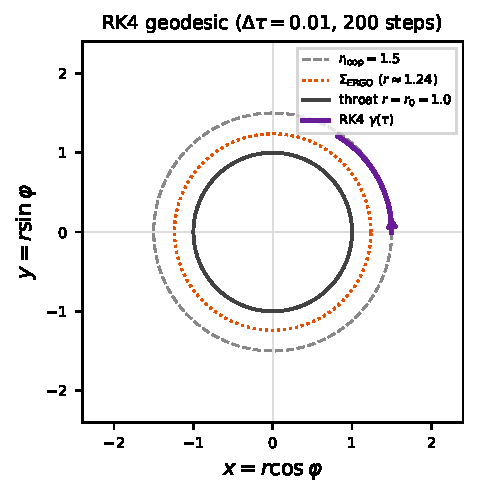
\includegraphics[width=\linewidth]{figures/geodesic_loop.pdf}
\caption{Equatorial projection of an RK4 co-rotating timelike geodesic $\gamma(\tau)$ initialized at $r_{\mathrm{loop}}=1.5\,r_{0}$ (reference profile), with throat and ergosurface $\Sigma_{\mathrm{ERGO}}$ ($g_{tt}=0$) indicated. The discrete monodromy proxy of Sec.~\ref{sec:monodromy} samples the distinct spacelike azimuthal circle ($g_{\varphi\varphi}>0$) at the same radius; neither curve is claimed to be a closed timelike curve.}
\label{fig:geodesic}
\end{minipage}
\end{figure}

%==============================================================================
\section{Symbolic Einstein tensor and energy conditions}
\label{sec:energy}

Einstein's equations read $\Gmn=\Rmn-\tfrac12 R\,g_{\mu\nu}=8\pi\Tmn$.
The equatorial components of $\Gmn$ and the associated NEC/WEC contractions are obtained by symbolic differentiation (Appendices~\ref{app:tensors}--\ref{app:energy}) and treated as \emph{background constraints} on the profile class~\eqref{eq:profiles}.
They are not assembled dynamically from curvature inside the discrete-transport analysis; numerical validation checks exercise only the corresponding quadratic contractions as consistency diagnostics.

\IfFileExists{derived_equations_summary.tex}{% Main-body summary (criterion C2: symbolic background constraints)
Substituting the explicit profiles~\eqref{eq:profiles} on the equatorial slice ($\theta=\pi/2$), 5 components of $\Gmn$ are non-zero: $G_{tt}$, $G_{t\varphi}$, $G_{rr}$, $G_{\theta\theta}$, and $G_{\varphi\varphi}$.
The effective stress-energy $\Tmn=\Gmn/(8\pi)$ is obtained by symbolic differentiation as a static background constraint (criterion~C2); it is not assembled dynamically from the discrete-transport analysis.
Key scalar invariants are
\begin{align}
\det(g_{\mu\nu}) &= -\frac{r^{5} e^{2\Phi(r)}}{r - b(r)}, \quad b(r)=r_{0} \left(\frac{r_{0}}{r}\right)^{\gamma}, \nonumber\\
R &= \mathcal{R}(\gamma,\alpha,\omega_0,\beta;r,r_0)\quad\text{(explicit form in Appendix~\ref{app:tensors})}.
\end{align}
The radial component $G_{rr}$ admits a compact closed form; all component expansions appear in Appendix~\ref{app:tensors}.
}{}
\IfFileExists{energy_conditions_summary.tex}{% Main-body summary (criterion C2: symbolic background constraints)
We evaluate the null and weak energy conditions~\cite{HawkingEllis1973,Visser1995} as
\emph{static background constraints} on the profile class: NEC requires
$\Tmn k^{\mu}k^{\nu}\ge 0$ for all null $k^{\mu}$; WEC requires
$\Tmn u^{\mu}u^{\nu}\ge 0$ for timelike $u^{\mu}$.
For a null vector with $k^{\varphi}=1$ and $g_{\mu\nu}k^{\mu}k^{\nu}=0$,
\begin{equation}
  k^t = \frac{r}{r \omega{\left(r \right)} - e^{\Phi{\left(r \right)}}}.
\end{equation}
With profiles~\eqref{eq:profiles}, the symbolically obtained lab-frame density admits a
negative throat limit $\lim_{r\to r_0^{+}}\rho$, consistent with exotic stress-energy
near the wormhole throat for this family; a full radial localization theorem is
\emph{not} claimed as a numerically established result.
Within an effective-field-theory (EFT) mean-field envelope, the non-minimal coupling
$\zeta\,\phif R$ is treated as a background parameter in
$\{\gamma,\alpha,\omega_{0},\beta,\zeta\}$ that can energetically bound local
NEC/WEC violations whenever $|\zeta\,\phif R|>|\rho_{\mathrm{neg}}|$.
Full NEC, WEC, and $\rho$ contractions are given in Appendix~\ref{app:energy}.
}{}

Within an EFT mean-field envelope, the non-minimal coupling $\zeta\,\phif R$ is regarded as a background parameter that can energetically bound local NEC/WEC violations whenever $|\zeta\,\phif R|$ exceeds the magnitude of the negative-energy density implied by $\Tmn=\Gmn/(8\pi)$.
This defines a self-consistent parameter domain for the profile class; it does not constitute a dynamical generation mechanism for exotic matter, nor a numerically established localization theorem.

%==============================================================================
\section{Discrete monodromy proxy and spectral diagnostics}
\label{sec:monodromy}

We construct a discrete transport operator by sampling a retarded kernel on the spacelike azimuthal circle of Sec.~\ref{sec:geometry} at fixed $(r,\theta)=(r_{\mathrm{loop}},\pi/2)$, where $g_{\varphi\varphi}>0$.
The massive Klein--Gordon equation on~\eqref{eq:metric},
\begin{equation}
\label{eq:kg}
\frac{1}{\sqrt{-g}}\,\partial_{\mu}\!\Bigl(\sqrt{-g}\,g^{\mu\nu}\partial_{\nu}\phi\Bigr)-m^{2}\phi=0,
\end{equation}
motivates the mode-augmented mass gap entering the kernel, but we do \emph{not} discretize the full curved-space PDE.
Instead we assemble finite matrices $K$ and $\widetilde{K}$ on that stationary spacelike circle.
On the uniform periodic $N$-node grid the sampled kernels are circulant, so their eigenvalues and spectral radii are the natural discrete-Fourier / spectral-method diagnostics for periodic mesh operators~\cite{Trefethen2000}.
Row-sum renormalization makes the control gate $K$ algebraically contractive; the infrared spectral diagnostic is the transition of the \emph{unnormalized} proxy $\widetilde{K}$ when the mass gap is removed (Sec.~\ref{sec:mass-gap}).

\subsection{Continuous Yukawa proxy}

Decomposing into azimuthal modes $\phi\sim\psi_{\nu}(r)\,e^{i(\nu\varphi-\Omega t)}$ suggests a mode-augmented mass
\begin{equation}
\label{eq:m-star}
m_{\ast}^{2}=m^{2}+\nu^{2}/g_{\varphi\varphi},
\qquad
G(\Delta s)\sim\frac{m_{\ast}}{4\pi\Delta s}\,e^{-m_{\ast}\Delta s},
\end{equation}
for a retarded Yukawa-type kernel sampled along the spacelike azimuthal circle (proper arc length $s$).
Equation~\eqref{eq:m-star} is the continuous \emph{proxy} that motivates the discrete construction below; it is not claimed to be the exact retarded Green function of~\eqref{eq:kg} on~\eqref{eq:metric}.

\subsection{Discrete monodromy operator}

\begin{definition}[Discrete monodromy $\MN$]
\label{def:MN}
Fix $r=r_{\mathrm{loop}}$, $\theta=\pi/2$, and $N$ uniform nodes $\chi_{i}=2\pi i/N$ along the spacelike azimuthal circle~\eqref{eq:gphiphi}.
Let $\Delta\varphi=2\pi/N$ and $\Delta\ell=\sqrt{g_{\varphi\varphi}}\,\Delta\varphi$ as in~\eqref{eq:Delta-ell}.
For forward proper arc-length separations $\Delta s_{j\to i}$ along that circle, define the sampled kernel matrix
\begin{equation}
\label{eq:K-raw}
\widetilde{K}_{ij}
=
\begin{cases}
G(\Delta s_{j\to i})\,\Delta\ell, & i\neq j,\\
0, & i=j,
\end{cases}
\end{equation}
with $G$ from~\eqref{eq:m-star}.
The discrete monodromy operator is the \emph{row-sum renormalized} matrix
\begin{equation}
\label{eq:K-renorm}
K_{ij}
=
\widetilde{K}_{ij}\,
\frac{\exp(-m_{\ast}\Delta\ell)}{\sum_{k}\widetilde{K}_{ik}}
\qquad\bigl(\text{when the row sum is nonzero}\bigr),
\end{equation}
and $\MN:\mathbb{R}^{N}\to\mathbb{R}^{N}$ acts by $\Phi\mapsto K\Phi$.
\end{definition}

The default numerical parameters are $r_{\mathrm{loop}}=1.5\,r_{0}$, $m^{2}=1$, $\nu=1$, and $N=128$, with solver tolerance $\mathrm{tol}=10^{-12}$ and residual thresholds $10^{-8}$--$10^{-10}$ for the convergence checks.

\subsection{\texorpdfstring{Discrete $H^{1}$-proxy norm and the renormalized control gate}{Discrete H1-proxy norm and the renormalized control gate}}

On periodic samples $\Phi\in\mathbb{R}^{N}$ we use the discrete norms
\begin{align}
\label{eq:discrete-norms}
\|\Phi\|_{L^{2}}^{2}
&=
\frac1N\sum_{i=0}^{N-1}\Phi_{i}^{2},
\qquad
\|\Phi\|_{H^{1}}^{2}
=
\|\Phi\|_{L^{2}}^{2}
+
\|\delta\Phi\|_{L^{2}}^{2},
\end{align}
where $(\delta\Phi)_{i}=(\Phi_{i+1}-\Phi_{i-1})/2$ is the central difference on the index circle (a discrete $H^{1}$-proxy; not a continuum Sobolev norm on the sampling circle).
The $L^{2}$ operator norm of $K$ is estimated by power iteration; the discrete Sobolev lift used as a Lipschitz monitor is
\begin{equation}
\label{eq:discrete-sobolev}
L
\le
\|K\|_{L^{2}}\,
\Bigl(1+\frac{\pi\sqrt{2}}{N}\Bigr).
\end{equation}
The factor $\bigl(1+\pi\sqrt{2}/N\bigr)$ follows from the standard discrete interpolation inequality relating the central-difference seminorm~$\|\delta\Phi\|_{L^{2}}$ to~$\|\Phi\|_{L^{2}}$ for periodic grid functions on the $N$-node circle.

\begin{remark}[Algebraic contraction of the row-sum--normalized gate $K$]
\label{rem:renorm-gate}
By the row-sum construction~\eqref{eq:K-renorm}, whenever $m_{\ast}>0$ and every row sum is nonzero, each row of $K$ sums to $\exp(-m_{\ast}\Delta\ell)<1$.
Hence
\[
\rho(K)\le\exp(-m_{\ast}\Delta\ell)<1
\]
is an \emph{imposed algebraic property} of the normalization---a numerical control gate---and \emph{not} a dynamical discovery extracted from the Einstein equations, continuum Klein--Gordon evolution, or any continuum self-consistency principle on~\eqref{eq:metric}.
If, in addition, the discrete-$H^{1}$ monitor~\eqref{eq:discrete-sobolev} satisfies $L<1$ (as verified numerically for the reference parameters), the Banach fixed-point theorem supplies a unique $\Phi^{*}=K\Phi^{*}$ with geometrically convergent Picard iteration on $(\mathbb{R}^{N},\|\cdot\|_{H^{1}})$.
This remark concerns only the renormalized matrix $K$; the physically informative infrared diagnostic remains the unnormalized proxy $\widetilde{K}$ of Sec.~\ref{sec:mass-gap}.
\end{remark}

\paragraph{Numerical verification of the renormalized gate.}
\label{sec:numerical}
Definition~\ref{def:MN} and Remark~\ref{rem:renorm-gate} are corroborated by high-resolution numerical validation checks covering:
\begin{enumerate}
  \item[(i)] geometric metric invariants, flare-out, and ergosurface location for~\eqref{eq:ref-params};
  \item[(ii)] energy-condition quadratic contractions as consistency diagnostics;
  \item[(iii)] monodromy bounds $\|K\|_{L^{2}}<1$ and $L<1$;
  \item[(iv)] Banach--Picard convergence $\|\Phi^{*}-K\Phi^{*}\|_{2}<10^{-8}$ in fewer than $500$ iterations for $N\in\{32,64,128\}$;
  \item[(v)] classical fourth-order Runge--Kutta integration of the co-rotating timelike geodesic diagnostic with proper-time step $\Delta\tau=0.01$ over $200$ steps.
\end{enumerate}
These checks confirm the discrete contraction of the \emph{row-sum renormalized} operator~\eqref{eq:K-renorm}.
The primary physical result of criterion~(C3) is instead the spectral transition of the \emph{unnormalized} proxy~\eqref{eq:K-raw} under $m^{2}\to 0$, developed next.

\subsection{The mass-gap threshold and massless exponential proxy}
\label{sec:mass-gap}

Because row-sum renormalization~\eqref{eq:K-renorm} enforces $\rho(K)<1$ whenever $m_{\ast}>0$, that normalized gate is a useful numerical control but \emph{cannot} diagnose infrared failure of the unnormalized proxy.
The decisive spectral diagnostic is therefore the unnormalized discrete kernel $\widetilde{K}$ of~\eqref{eq:K-raw}, which we study on the reference loop $r_{\mathrm{loop}}=1.5\,r_{0}$ (equatorial $g_{\varphi\varphi}=r_{\mathrm{loop}}^{2}$) at azimuthal mode $\nu=0$, so that
\begin{equation}
\label{eq:m-star-nu0}
m_{\ast}=\sqrt{m^{2}}
\end{equation}
carries no angular mass gap.
Two proxy kernels on the one-dimensional azimuthal loop are compared under this protocol:
\begin{align}
\label{eq:kernels-path3}
G_{\mathrm{Y}}(\Delta s)
&=
\frac{m_{\ast}}{4\pi\Delta s}\,e^{-m_{\ast}\Delta s},
&
G_{\mathrm{E}}(\Delta s)
&=
e^{-m_{\ast}\Delta s}.
\end{align}
Here $G_{\mathrm{E}}$ is a \emph{massless exponential proxy} for discrete loop transport---a scalar kernel on the periodic one-dimensional loop, \emph{not} a three-dimensional Coulomb propagator.
As $m^{2}\to 0$ one has $G_{\mathrm{E}}\to 1$, whereas $G_{\mathrm{Y}}$ collapses by its prefactor $\propto m_{\ast}$ and therefore \emph{cannot} diagnose massless infrared failure of the discrete monodromy.

\paragraph{Constant off-diagonal kernel at $m^{2}=0$.}
At $m^{2}=0$ and $\nu=0$, the massless exponential proxy reduces to the constant off-diagonal circulant
\begin{equation}
\label{eq:massless-kernel}
\widetilde{K}_{ij}
=
\begin{cases}
\Delta\ell, & i\neq j,\\
0, & i=j,
\end{cases}
\qquad
\Delta\ell=\sqrt{g_{\varphi\varphi}}\,\frac{2\pi}{N}.
\end{equation}
Its spectrum is elementary: the constant mode has eigenvalue $(N-1)\Delta\ell$, while every mean-zero mode has eigenvalue $-\Delta\ell$.
Hence
\begin{equation}
\label{eq:massless-rho}
\rho\bigl(\widetilde{K}_{N}\bigr)
=
(N-1)\Delta\ell
=
2\pi\sqrt{g_{\varphi\varphi}}\,\frac{N-1}{N}
\;\xrightarrow{N\to\infty}\;
\rho_{\infty}
=
2\pi\sqrt{g_{\varphi\varphi}}.
\end{equation}
On the reference loop, $\sqrt{g_{\varphi\varphi}}=r_{\mathrm{loop}}=1.5$ and
\begin{equation}
\label{eq:rho-infty-num}
\rho_{\infty}=3\pi\approx 9.4248,
\end{equation}
which already exceeds unity by a wide margin.
Although the headline numerics are reported at $r_{\mathrm{loop}}=1.5\,r_{0}$, the massless spectral limit $\rho_{\infty}=2\pi\sqrt{g_{\varphi\varphi}}$ scales linearly with $\sqrt{g_{\varphi\varphi}}$ and the rupture $\rho_{\infty}>1$ therefore persists at any sampling radius where the discrete proxy is assembled.
Thus, for the massless exponential proxy, the constant off-diagonal kernel $\widetilde{K}$ is \emph{not} a contraction for any $N\ge 2$.

\begin{proposition}[Mass-gap threshold for discrete-proxy contractivity]
\label{prop:mass-gap}
Fix the reference profile~\eqref{eq:ref-params}, $r_{\mathrm{loop}}=1.5\,r_{0}$, and $\nu=0$.
Let $\widetilde{K}_{N}(m^{2})$ be the unnormalized massless-exponential monodromy~\eqref{eq:K-raw}--\eqref{eq:kernels-path3}.
\begin{enumerate}
  \item[(i)] \textbf{Massless phase.}
    If $m^{2}=0$, then $\rho(\widetilde{K}_{N})\to 2\pi\sqrt{g_{\varphi\varphi}}>1$.
    The Banach fixed-point argument fails for this proxy: discrete-proxy contractivity is \emph{not} guaranteed by contraction of $\widetilde{K}$.
  \item[(ii)] \textbf{Massive exponential phase.}
    For sufficiently large $m^{2}>0$, exponential screening restores $\rho(\widetilde{K}_{N})<1$ on the high-resolution grids reported below (numerical evidence for $m^{2}=1$).
  \item[(iii)] \textbf{Threshold.}
    There exists a critical mass gap $m_{c}^{2}\in(0,1)$ on this background such that
    \[
    \rho\bigl(\widetilde{K}_{N}(m^{2})\bigr)
    \;\ge\; 1
    \quad\text{for all }m^{2}\le m_{c}^{2}
    \text{ and }N\text{ large},
    \]
    while $\rho<1$ throughout the high-resolution grid when $m^{2}=1$.
\end{enumerate}
Consequently, a strictly positive mass gap is a \emph{necessary} structural ingredient for contractivity of the present unnormalized discrete proxy on the wormhole loop; the spectral transition of $\widetilde{K}$ as $m^{2}\downarrow 0$ defines the boundary of that contractivity regime.
\end{proposition}

\paragraph{Methodological caveat.}
The identity $\rho_{\infty}=2\pi\sqrt{g_{\varphi\varphi}}=3\pi$ on the reference loop is an \emph{exact} spectral limit of the constant off-diagonal discrete proxy~\eqref{eq:massless-kernel}--\eqref{eq:massless-rho}.
It is \emph{not} claimed to be an analytic continuum eigenvalue of the full curved-space Klein--Gordon operator~\eqref{eq:kg} on~\eqref{eq:metric}.
Finite-$N$ values $\rho(\widetilde{K}_{N})$ and Richardson-type extrapolations $\rho_{\infty}^{\mathrm{extrap}}$ reported below likewise characterize the discrete loop proxy, not a closed-form continuum Green function.

\paragraph{Numerical continuum campaign.}
Assembling the unnormalized proxy without row-sum renormalization, we sweep
\[
N\in\{32,64,128,256,512,1024\},
\qquad
m^{2}\in\{1,10^{-2},10^{-4},10^{-8},10^{-12},0\}
\]
at $\nu=0$.
Representative high-resolution values for $G_{\mathrm{E}}$ are
\begin{equation}
\label{eq:path3-numbers}
\begin{aligned}
m^{2}=1:&\quad
\rho(512)=0.9907,\;
\rho(1024)=0.9953,\;
\rho_{\infty}^{\mathrm{extrap}}\simeq 0.9999<1,\\[2pt]
m^{2}=10^{-2}:&\quad
\rho(1024)\simeq 6.097>1,\\[2pt]
m^{2}\to 0:&\quad
\rho(1024)\simeq 9.416
\;\to\;
3\pi,
\end{aligned}
\end{equation}
in quantitative agreement with the constant off-diagonal limit~\eqref{eq:massless-rho}--\eqref{eq:rho-infty-num}.
Thus the growing trend of $\rho(N)$ observed at moderate resolution \emph{does} cross the contractivity threshold once the mass gap is removed, rather than saturating below unity.
(The extrapolated value $\rho_{\infty}^{\mathrm{extrap}}\simeq 0.9999$ at $m^{2}=1$ lies close to the threshold and should be read as a high-resolution proxy diagnostic, not as an exact continuum eigenvalue.)
By contrast, the Yukawa family $G_{\mathrm{Y}}$ remains contractive on the entire grid and collapses to $\rho\to 0$ as $m^{2}\to 0$, confirming that its prefactor masks the massless spectral rupture of $G_{\mathrm{E}}$ and must not be used as the infrared diagnostic.

\paragraph{Spectral reading of the proxy and infrared threshold.}
On this Morris--Thorne spacelike loop, existence of a unique attractive fixed point of the unnormalized discrete transport map is guaranteed by contraction only inside the massive phase $\rho(\widetilde{K})<1$.
Crossing into the massless phase $\rho\ge 1$ means that loop transport ceases to be a contraction: Picard iteration need not converge and uniqueness of a fixed point is no longer enforced by the spectral radius of this discrete kernel.
The mass-gap threshold $m_{c}^{2}$ is therefore the \emph{infrared frontier of contractivity} for the present discrete monodromy proxy on the wormhole background under study.
The discrete-monodromy source code and full spectral tables accompanying this work are available at \url{https://github.com/mauramyrez/ctc-discrete-monodromy}; the Path-3 continuum campaign report is archived as \texttt{docs/path3\_continuum\_report.md} in that repository.

%==============================================================================
\section{Conclusion}
\label{sec:conclusion}

We have analyzed the spectral structure of a discrete spacelike azimuthal-transport proxy on axisymmetric frame-dragging Morris--Thorne backgrounds.
The sampling circle at fixed $(r,\theta)$ is spacelike ($g_{\varphi\varphi}>0$); the certified statements concern finite matrices $K$ and $\widetilde{K}$, not continuum closed-timelike-curve field theorems.
Row-sum renormalization yields a contractive discrete-proxy gate by algebraic design (Remark~\ref{rem:renorm-gate}); the central spectral conclusion concerns instead the unnormalized massless exponential proxy $\widetilde{K}$: removing the mass gap drives its discrete-proxy spectral radius through
$\rho(\widetilde{K})\to 2\pi\sqrt{g_{\varphi\varphi}}\simeq 9.42>1$,
so that discrete-proxy contractivity fails in the massless infrared on the reference wormhole loop.
This $\rho_{\infty}=3\pi$ limit characterizes the constant off-diagonal discrete proxy on the loop and is not claimed as an exact continuum eigenvalue of a full curved-space Klein--Gordon simulation.

In terms of the criteria~(C1)--(C3):
\begin{itemize}
  \item \textbf{(C1)} Explicit profiles~\eqref{eq:profiles} with flare-out, reference parameters~\eqref{eq:ref-params}, and equatorial ergoregion~\eqref{eq:ergo-open} bounded by $\Sigma_{\mathrm{ERGO}}$ (where $g_{tt}>0$), corroborated by metric invariants and co-rotating geodesic diagnostics.
  \item \textbf{(C2)} Symbolically differentiated equatorial $\Gmn$ and NEC/WEC contractions as static background constraints (Appendices~\ref{app:tensors}--\ref{app:energy}), not dynamically generated from the discrete-transport map.
  \item \textbf{(C3)} Algebraic contraction of the row-sum--normalized gate by design (Remark~\ref{rem:renorm-gate}), together with the unnormalized mass-gap threshold and massless spectral rupture of the exponential proxy (Proposition~\ref{prop:mass-gap}, Sec.~\ref{sec:mass-gap}), including the exact discrete limit $\rho_{\infty}=3\pi$ on the reference loop.
\end{itemize}

The presence of an ergoregion does not by itself restore or destroy global hyperbolicity; the present spectral diagnostics remain those of a spacelike loop-transport proxy on a fixed stationary background.
Dynamical (non-stationary) perturbations of $\omegar$ are left for future work.

\paragraph{Heuristic semiclassical outlook.}
Beyond the discrete spectral analysis, one may speculate that a curvature-referenced microscopic scale could eventually regulate short-distance vacuum polarization near $\Sigma_{\mathrm{ERGO}}$ in a non-minimally coupled scalar sector~\cite{KimThorne1991,Hawking1992,KayRadzikowskiWald1997}.
We record this only as an informal outlook: no Hadamard parametrix is constructed here, no bound on $\langle\Tmn\rangle_{\mathrm{ren}}$ is proved, and no claim is made that non-minimal coupling evades known no-go results for Hadamard states near compactly generated Cauchy horizons.
Such questions lie outside the certified scope of criteria~(C1)--(C3).

\section*{Conflict of interest statement}
The authors declare that there are no conflicts of interest regarding the publication of this paper.

\section*{Ethical statement}
This research did not involve human participants, animal subjects, or sensitive data collection; thus, ethical approval was not required.

\section*{Funding statement}
This work received no specific grant from any funding agency in the public, commercial, or not-for-profit sectors.

\ack{The discrete-monodromy source code and full spectral tables accompanying this work are available at \url{https://github.com/mauramyrez/ctc-discrete-monodromy}; the Path-3 continuum campaign report is archived as \texttt{docs/path3\_continuum\_report.md} in that repository.}

\data{The discrete monodromy diagnostics and Path-3 spectral tables supporting this work are openly available at \url{https://github.com/mauramyrez/ctc-discrete-monodromy}.}

\suppdata{The Path-3 continuum campaign report is archived as \texttt{docs/path3\_continuum\_report.md} in the companion repository.}

%==============================================================================
\appendix

\section{Full equatorial Einstein tensor components}
\label{app:tensors}

Substituting~\eqref{eq:profiles} at $\theta=\pi/2$, the non-zero components of $\Gmn$ and the Ricci scalar $R$ are collected below.
Repeated factors are abbreviated for typographic clarity; the expansions are algebraically identical to the symbolic differentiation used for criterion~(C2).
\IfFileExists{appendix_tensor_components.tex}{% Appendix A — equatorial Einstein tensor (profiles substituted; θ=π/2)
% Algebraically identical to the symbolic output of scripts/derive_tensors.py;
% reformatted with auxiliary notation and term-by-term line breaks for CQG (interim RevTeX source).

\paragraph{Auxiliary notation.}
To keep the expansions within the page width we write
\begin{equation}
\xi\equiv\Bigl(\frac{r_{0}}{r}\Bigr)^{\!\gamma},\qquad
E_{\alpha}\equiv e^{\alpha r_{0}/r},\qquad
E_{\beta}\equiv e^{\beta r/r_{0}}.
\end{equation}

\begin{subequations}
\paragraph{$G_{tt}$.}
\begin{align}
G_{tt}
&=
\frac{e^{-12\beta}}{4\,r^{11}r_{0}^{5}\,
\exp\!\bigl(4\alpha r_{0}/r+12\beta r/r_{0}-12\beta\bigr)}
\,N_{tt},
\\
\begin{split}
N_{tt}
&=
  4\alpha^{2}\omega_{0}^{2} r^{9} r_{0}^{7}\,e^{2\beta}\,E_{\alpha}^{4}\,E_{\beta}^{10}
\\&\quad
- 4\alpha^{2}\omega_{0}^{2} r^{8} r_{0}^{8}\,\xi\,e^{2\beta}\,E_{\alpha}^{4}\,E_{\beta}^{10}
\\&\quad
- 4\alpha\beta\omega_{0}^{2} r^{11} r_{0}^{5}\,e^{2\beta}\,E_{\alpha}^{4}\,E_{\beta}^{10}
\\&\quad
+ 4\alpha\beta\omega_{0}^{2} r^{10} r_{0}^{6}\,\xi\,e^{2\beta}\,E_{\alpha}^{4}\,E_{\beta}^{10}
\\&\quad
+ 2\alpha\gamma\omega_{0}^{2} r^{9} r_{0}^{7}\,\xi\,e^{2\beta}\,E_{\alpha}^{4}\,E_{\beta}^{10}
\\&\quad
- 4\alpha\omega_{0}^{2} r^{10} r_{0}^{6}\,e^{2\beta}\,E_{\alpha}^{4}\,E_{\beta}^{10}
\\&\quad
+ 6\alpha\omega_{0}^{2} r^{9} r_{0}^{7}\,\xi\,e^{2\beta}\,E_{\alpha}^{4}\,E_{\beta}^{10}
\\&\quad
- 3\beta^{2}\omega_{0}^{4} r^{15} r_{0}^{3}\,e^{4\beta}\,E_{\alpha}^{6}\,E_{\beta}^{8}
\\&\quad
+ 3\beta^{2}\omega_{0}^{4} r^{14} r_{0}^{4}\,\xi\,e^{4\beta}\,E_{\alpha}^{6}\,E_{\beta}^{8}
\\&\quad
- 5\beta^{2}\omega_{0}^{2} r^{13} r_{0}^{3}\,e^{2\beta}\,E_{\alpha}^{4}\,E_{\beta}^{10}
\\&\quad
+ 5\beta^{2}\omega_{0}^{2} r^{12} r_{0}^{4}\,\xi\,e^{2\beta}\,E_{\alpha}^{4}\,E_{\beta}^{10}
\\&\quad
+ 2\beta\gamma\omega_{0}^{2} r^{11} r_{0}^{5}\,\xi\,e^{2\beta}\,E_{\alpha}^{4}\,E_{\beta}^{10}
\\&\quad
+ 16\beta\omega_{0}^{2} r^{12} r_{0}^{4}\,e^{2\beta}\,E_{\alpha}^{4}\,E_{\beta}^{10}
\\&\quad
- 14\beta\omega_{0}^{2} r^{11} r_{0}^{5}\,\xi\,e^{2\beta}\,E_{\alpha}^{4}\,E_{\beta}^{10}
\\&\quad
+ 2\gamma\omega_{0}^{2} r^{10} r_{0}^{6}\,\xi\,e^{2\beta}\,E_{\alpha}^{4}\,E_{\beta}^{10}
\\&\quad
- 4\gamma r^{8} r_{0}^{6}\,\xi\,E_{\alpha}^{2}\,E_{\beta}^{12}
\\&\quad
+ 2\omega_{0}^{2} r^{10} r_{0}^{6}\,\xi\,e^{2\beta}\,E_{\alpha}^{4}\,E_{\beta}^{10}
\\&\quad
- 4 r^{9} r_{0}^{5}\,E_{\alpha}^{2}\,E_{\beta}^{12}.
\end{split}
\end{align}

\paragraph{$G_{t\varphi}$.}
\begin{multline}
G_{t\varphi}
=
\frac{1}{4\,r^{3}r_{0}^{2}\,
\exp\!\bigl[\beta(3r-r_{0})/r_{0}\bigr]}
\Bigl[
-4\alpha^{2}\omega_{0}\,r\,r_{0}^{4}\,E_{\beta}^{2}
+4\alpha^{2}\omega_{0}\,r_{0}^{5}\,\xi\,E_{\beta}^{2}
\\
\quad
+2\alpha\beta\omega_{0}\,r^{3}r_{0}^{2}\,E_{\beta}^{2}
-2\alpha\beta\omega_{0}\,r^{2}r_{0}^{3}\,\xi\,E_{\beta}^{2}
-2\alpha\gamma\omega_{0}\,r\,r_{0}^{4}\,\xi\,E_{\beta}^{2}
\\
\quad
+4\alpha\omega_{0}\,r^{2}r_{0}^{3}\,E_{\beta}^{2}
-6\alpha\omega_{0}\,r\,r_{0}^{4}\,\xi\,E_{\beta}^{2}
+3\beta^{2}\omega_{0}^{3}\,r^{7}\,e^{2\beta}\,E_{\alpha}^{2}
\\
\quad
-3\beta^{2}\omega_{0}^{3}\,r^{6}r_{0}\,\xi\,e^{2\beta}\,E_{\alpha}^{2}
+2\beta^{2}\omega_{0}\,r^{5}\,E_{\beta}^{2}
-2\beta^{2}\omega_{0}\,r^{4}r_{0}\,\xi\,E_{\beta}^{2}
\\
\quad
-\beta\gamma\omega_{0}\,r^{3}r_{0}^{2}\,\xi\,E_{\beta}^{2}
-8\beta\omega_{0}\,r^{4}r_{0}\,E_{\beta}^{2}
+7\beta\omega_{0}\,r^{3}r_{0}^{2}\,\xi\,E_{\beta}^{2}
\\
\quad
-2\gamma\omega_{0}\,r^{2}r_{0}^{3}\,\xi\,E_{\beta}^{2}
-2\omega_{0}\,r^{2}r_{0}^{3}\,\xi\,E_{\beta}^{2}
\Bigr].
\end{multline}

\paragraph{$G_{rr}$.}
\begin{equation}
G_{rr}
=
\frac{1}{4\,r^{5}r_{0}^{2}}
\Bigl[
8\alpha\,r^{2}r_{0}^{3}
+4\,r^{3}r_{0}^{2}
+\beta^{2}\omega_{0}^{2}\,r^{7}\,e^{2\beta}\,E_{\alpha}^{2}\,E_{\beta}^{-2}
\Bigr].
\end{equation}

\paragraph{$G_{\theta\theta}$.}
\begin{multline}
G_{\theta\theta}
=
\frac{E_{\beta}^{-2}}{4\,r^{6}r_{0}^{2}}
\Bigl[
4\alpha^{2}\,r^{4}r_{0}^{4}\,E_{\beta}^{2}
-4\alpha^{2}\,r^{3}r_{0}^{5}\,\xi\,E_{\beta}^{2}
+2\alpha\gamma\,r^{4}r_{0}^{4}\,\xi\,E_{\beta}^{2}
\\
\quad
-4\alpha\,r^{5}r_{0}^{3}\,E_{\beta}^{2}
+6\alpha\,r^{4}r_{0}^{4}\,\xi\,E_{\beta}^{2}
-\beta^{2}\omega_{0}^{2}\,r^{10}\,e^{2\beta}\,E_{\alpha}^{2}
\\
\quad
+\beta^{2}\omega_{0}^{2}\,r^{9}r_{0}\,\xi\,e^{2\beta}\,E_{\alpha}^{2}
+2\gamma\,r^{5}r_{0}^{3}\,\xi\,E_{\beta}^{2}
+2\,r^{5}r_{0}^{3}\,\xi\,E_{\beta}^{2}
\Bigr].
\end{multline}

\paragraph{$G_{\varphi\varphi}$.}
\begin{multline}
G_{\varphi\varphi}
=
\frac{E_{\beta}^{-2}}{4\,r^{6}r_{0}^{2}}
\Bigl[
4\alpha^{2}\,r^{4}r_{0}^{4}\,E_{\beta}^{2}
-4\alpha^{2}\,r^{3}r_{0}^{5}\,\xi\,E_{\beta}^{2}
+2\alpha\gamma\,r^{4}r_{0}^{4}\,\xi\,E_{\beta}^{2}
\\
\quad
-4\alpha\,r^{5}r_{0}^{3}\,E_{\beta}^{2}
+6\alpha\,r^{4}r_{0}^{4}\,\xi\,E_{\beta}^{2}
-3\beta^{2}\omega_{0}^{2}\,r^{10}\,e^{2\beta}\,E_{\alpha}^{2}
\\
\quad
+3\beta^{2}\omega_{0}^{2}\,r^{9}r_{0}\,\xi\,e^{2\beta}\,E_{\alpha}^{2}
+2\gamma\,r^{5}r_{0}^{3}\,\xi\,E_{\beta}^{2}
+2\,r^{5}r_{0}^{3}\,\xi\,E_{\beta}^{2}
\Bigr].
\end{multline}

\paragraph{Ricci scalar.}
\begin{multline}
R
=
\frac{E_{\beta}^{-2}}{2\,r^{14}r_{0}^{2}}
\Bigl[
-4\alpha^{2}\,r^{10}r_{0}^{4}\,E_{\beta}^{2}
+4\alpha^{2}\,r^{9}r_{0}^{5}\,\xi\,E_{\beta}^{2}
-2\alpha\gamma\,r^{10}r_{0}^{4}\,\xi\,E_{\beta}^{2}
\\
\quad
-2\alpha\,r^{10}r_{0}^{4}\,\xi\,E_{\beta}^{2}
+\beta^{2}\omega_{0}^{2}\,r^{16}\,e^{2\beta}\,E_{\alpha}^{2}
-\beta^{2}\omega_{0}^{2}\,r^{15}r_{0}\,\xi\,e^{2\beta}\,E_{\alpha}^{2}
\\
\quad
-4\gamma\,r^{11}r_{0}^{3}\,\xi\,E_{\beta}^{2}
-4\,r^{12}r_{0}^{2}\,E_{\beta}^{2}
\Bigr].
\end{multline}
\end{subequations}
}{}

\section{Energy condition contractions}
\label{app:energy}

Null (NEC) and weak (WEC) contractions with the same profiles, treated as static background constraints rather than dynamically evolved stress-energy:
\IfFileExists{appendix_energy_conditions.tex}{% Appendix B — NEC / WEC / ρ contractions (profiles substituted)
% Algebraically identical to scripts/verify_energy_conditions.py;
% reformatted with the auxiliary notation of Appendix~\ref{app:tensors}.

Recall $\xi\equiv(r_{0}/r)^{\gamma}$,
$E_{\alpha}\equiv e^{\alpha r_{0}/r}$,
and $E_{\beta}\equiv e^{\beta r/r_{0}}$.

\begin{subequations}
\paragraph{Null energy condition.}
\begin{multline}
T_{\mu\nu}k^{\mu}k^{\nu}
=
\frac{1}{16\pi\,r^{3}r_{0}^{2}
\bigl(\omega_{0}\,r\,e^{\alpha r_{0}/r+\beta}-E_{\beta}\bigr)^{2}}
\,N_{\mathrm{NEC}},
\end{multline}
\begin{align}
\begin{split}
N_{\mathrm{NEC}}
&=
  2\alpha^{2}\,r\,r_{0}^{4}\,E_{\beta}^{2}
- 2\alpha^{2}\,r_{0}^{5}\,\xi\,E_{\beta}^{2}
\\&\quad
- 2\alpha\beta\omega_{0}\,r^{4}r_{0}^{2}\,e^{\beta}\,E_{\alpha}\,E_{\beta}
+ 2\alpha\beta\omega_{0}\,r^{3}r_{0}^{3}\,\xi\,e^{\beta}\,E_{\alpha}\,E_{\beta}
\\&\quad
+ \alpha\gamma\,r\,r_{0}^{4}\,\xi\,E_{\beta}^{2}
- 2\alpha\,r^{2}r_{0}^{3}\,E_{\beta}^{2}
+ 3\alpha\,r\,r_{0}^{4}\,\xi\,E_{\beta}^{2}
\\&\quad
- 2\beta^{2}\omega_{0}^{2}\,r^{7}\,e^{2\beta}\,E_{\alpha}^{2}
+ 2\beta^{2}\omega_{0}^{2}\,r^{6}r_{0}\,\xi\,e^{2\beta}\,E_{\alpha}^{2}
\\&\quad
- 2\beta^{2}\omega_{0}\,r^{6}\,e^{\beta}\,E_{\alpha}\,E_{\beta}
+ 2\beta^{2}\omega_{0}\,r^{5}r_{0}\,\xi\,e^{\beta}\,E_{\alpha}\,E_{\beta}
\\&\quad
+ \beta\gamma\omega_{0}\,r^{4}r_{0}^{2}\,\xi\,e^{\beta}\,E_{\alpha}\,E_{\beta}
+ 8\beta\omega_{0}\,r^{5}r_{0}\,e^{\beta}\,E_{\alpha}\,E_{\beta}
\\&\quad
- 7\beta\omega_{0}\,r^{4}r_{0}^{2}\,\xi\,e^{\beta}\,E_{\alpha}\,E_{\beta}
- \gamma\,r^{2}r_{0}^{3}\,\xi\,E_{\beta}^{2}
\\&\quad
- 2\,r^{3}r_{0}^{2}\,E_{\beta}^{2}
+ r^{2}r_{0}^{3}\,\xi\,E_{\beta}^{2}.
\end{split}
\end{align}

\paragraph{Weak energy condition.}
\begin{align}
T_{\mu\nu}u^{\mu}u^{\nu}
&=
\frac{E_{\beta}^{-2}}{32\pi\,r^{3}r_{0}^{2}
\bigl(\omega_{0}^{2}r^{2}\,e^{2\alpha r_{0}/r+2\beta}-E_{\beta}^{2}\bigr)}
\,N_{\mathrm{WEC}},
\\
\begin{split}
N_{\mathrm{WEC}}
&=
- 4\alpha^{2}\omega_{0}^{2}\,r\,r_{0}^{4}\,e^{2\beta}\,E_{\alpha}^{2}\,E_{\beta}^{2}
+ 4\alpha^{2}\omega_{0}^{2}\,r_{0}^{5}\,\xi\,e^{2\beta}\,E_{\alpha}^{2}\,E_{\beta}^{2}
\\&\quad
+ 4\alpha\beta\omega_{0}^{2}\,r^{3}r_{0}^{2}\,e^{2\beta}\,E_{\alpha}^{2}\,E_{\beta}^{2}
- 4\alpha\beta\omega_{0}^{2}\,r^{2}r_{0}^{3}\,\xi\,e^{2\beta}\,E_{\alpha}^{2}\,E_{\beta}^{2}
\\&\quad
- 2\alpha\gamma\omega_{0}^{2}\,r\,r_{0}^{4}\,\xi\,e^{2\beta}\,E_{\alpha}^{2}\,E_{\beta}^{2}
+ 4\alpha\omega_{0}^{2}\,r^{2}r_{0}^{3}\,e^{2\beta}\,E_{\alpha}^{2}\,E_{\beta}^{2}
\\&\quad
- 6\alpha\omega_{0}^{2}\,r\,r_{0}^{4}\,\xi\,e^{2\beta}\,E_{\alpha}^{2}\,E_{\beta}^{2}
+ 3\beta^{2}\omega_{0}^{4}\,r^{7}\,e^{4\beta}\,E_{\alpha}^{4}
\\&\quad
- 3\beta^{2}\omega_{0}^{4}\,r^{6}r_{0}\,\xi\,e^{4\beta}\,E_{\alpha}^{4}
+ 5\beta^{2}\omega_{0}^{2}\,r^{5}\,e^{2\beta}\,E_{\alpha}^{2}\,E_{\beta}^{2}
\\&\quad
- 5\beta^{2}\omega_{0}^{2}\,r^{4}r_{0}\,\xi\,e^{2\beta}\,E_{\alpha}^{2}\,E_{\beta}^{2}
- 2\beta\gamma\omega_{0}^{2}\,r^{3}r_{0}^{2}\,\xi\,e^{2\beta}\,E_{\alpha}^{2}\,E_{\beta}^{2}
\\&\quad
- 16\beta\omega_{0}^{2}\,r^{4}r_{0}\,e^{2\beta}\,E_{\alpha}^{2}\,E_{\beta}^{2}
+ 14\beta\omega_{0}^{2}\,r^{3}r_{0}^{2}\,\xi\,e^{2\beta}\,E_{\alpha}^{2}\,E_{\beta}^{2}
\\&\quad
- 2\gamma\omega_{0}^{2}\,r^{2}r_{0}^{3}\,\xi\,e^{2\beta}\,E_{\alpha}^{2}\,E_{\beta}^{2}
+ 4\gamma\,r_{0}^{3}\,\xi\,E_{\beta}^{4}
\\&\quad
- 2\omega_{0}^{2}\,r^{2}r_{0}^{3}\,\xi\,e^{2\beta}\,E_{\alpha}^{2}\,E_{\beta}^{2}
+ 4\,r\,r_{0}^{2}\,E_{\beta}^{4}.
\end{split}
\end{align}

\paragraph{Lab-frame energy density.}
\begin{align}
\rho
\equiv
T_{\mu\nu}u^{\mu}u^{\nu}\big|_{u=\partial_{t}}
&=
\frac{E_{\alpha}^{-2}\,E_{\beta}^{-4}}{32\pi\,r^{3}r_{0}^{2}}
\,N_{\rho},
\\
\begin{split}
N_{\rho}
&=
  4\alpha^{2}\omega_{0}^{2}\,r\,r_{0}^{4}\,e^{2\beta}\,E_{\alpha}^{2}\,E_{\beta}^{2}
- 4\alpha^{2}\omega_{0}^{2}\,r_{0}^{5}\,\xi\,e^{2\beta}\,E_{\alpha}^{2}\,E_{\beta}^{2}
\\&\quad
- 4\alpha\beta\omega_{0}^{2}\,r^{3}r_{0}^{2}\,e^{2\beta}\,E_{\alpha}^{2}\,E_{\beta}^{2}
+ 4\alpha\beta\omega_{0}^{2}\,r^{2}r_{0}^{3}\,\xi\,e^{2\beta}\,E_{\alpha}^{2}\,E_{\beta}^{2}
\\&\quad
+ 2\alpha\gamma\omega_{0}^{2}\,r\,r_{0}^{4}\,\xi\,e^{2\beta}\,E_{\alpha}^{2}\,E_{\beta}^{2}
- 4\alpha\omega_{0}^{2}\,r^{2}r_{0}^{3}\,e^{2\beta}\,E_{\alpha}^{2}\,E_{\beta}^{2}
\\&\quad
+ 6\alpha\omega_{0}^{2}\,r\,r_{0}^{4}\,\xi\,e^{2\beta}\,E_{\alpha}^{2}\,E_{\beta}^{2}
- 3\beta^{2}\omega_{0}^{4}\,r^{7}\,e^{4\beta}\,E_{\alpha}^{4}
\\&\quad
+ 3\beta^{2}\omega_{0}^{4}\,r^{6}r_{0}\,\xi\,e^{4\beta}\,E_{\alpha}^{4}
- 5\beta^{2}\omega_{0}^{2}\,r^{5}\,e^{2\beta}\,E_{\alpha}^{2}\,E_{\beta}^{2}
\\&\quad
+ 5\beta^{2}\omega_{0}^{2}\,r^{4}r_{0}\,\xi\,e^{2\beta}\,E_{\alpha}^{2}\,E_{\beta}^{2}
+ 2\beta\gamma\omega_{0}^{2}\,r^{3}r_{0}^{2}\,\xi\,e^{2\beta}\,E_{\alpha}^{2}\,E_{\beta}^{2}
\\&\quad
+ 16\beta\omega_{0}^{2}\,r^{4}r_{0}\,e^{2\beta}\,E_{\alpha}^{2}\,E_{\beta}^{2}
- 14\beta\omega_{0}^{2}\,r^{3}r_{0}^{2}\,\xi\,e^{2\beta}\,E_{\alpha}^{2}\,E_{\beta}^{2}
\\&\quad
+ 2\gamma\omega_{0}^{2}\,r^{2}r_{0}^{3}\,\xi\,e^{2\beta}\,E_{\alpha}^{2}\,E_{\beta}^{2}
- 4\gamma\,r_{0}^{3}\,\xi\,E_{\beta}^{4}
\\&\quad
+ 2\omega_{0}^{2}\,r^{2}r_{0}^{3}\,\xi\,e^{2\beta}\,E_{\alpha}^{2}\,E_{\beta}^{2}
- 4\,r\,r_{0}^{2}\,E_{\beta}^{4}.
\end{split}
\end{align}

\paragraph{Throat limit ($r\to r_{0}^{+}$).}
The throat value is the continuous evaluation of the preceding density,
\begin{equation}
\lim_{r\to r_{0}^{+}}\rho
=
\frac{E_{\alpha}^{-2}\,E_{\beta}^{-4}}{32\pi\,r^{3}r_{0}^{2}}
\,N_{\rho}
\Big|_{r=r_{0}},
\end{equation}
with $\xi\big|_{r=r_{0}}=1$ and $E_{\alpha}\big|_{r=r_{0}}=e^{\alpha}$,
$E_{\beta}\big|_{r=r_{0}}=e^{\beta}$.

\paragraph{Scalar-tensor bounding.}
With non-minimal coupling $\zeta\,\phif R$,
\begin{multline}
\rho_{\mathrm{neg}}+\zeta\,\phif R
=
\frac{E_{\beta}^{-2}}{2\,r^{14}r_{0}^{2}}
\Bigl[
-4\alpha^{2}\,\phif\,\zeta\,r^{10}r_{0}^{4}\,E_{\beta}^{2}
+4\alpha^{2}\,\phif\,\zeta\,r^{9}r_{0}^{5}\,\xi\,E_{\beta}^{2}
\\
\quad
-2\alpha\gamma\,\phif\,\zeta\,r^{10}r_{0}^{4}\,\xi\,E_{\beta}^{2}
-2\alpha\,\phif\,\zeta\,r^{10}r_{0}^{4}\,\xi\,E_{\beta}^{2}
\\
\quad
+\beta^{2}\omega_{0}^{2}\,\phif\,\zeta\,r^{16}\,e^{2\beta}\,E_{\alpha}^{2}
-\beta^{2}\omega_{0}^{2}\,\phif\,\zeta\,r^{15}r_{0}\,\xi\,e^{2\beta}\,E_{\alpha}^{2}
\\
\quad
-4\gamma\,\phif\,\zeta\,r^{11}r_{0}^{3}\,\xi\,E_{\beta}^{2}
-4\,\phif\,\zeta\,r^{12}r_{0}^{2}\,E_{\beta}^{2}
+2\,r^{14}r_{0}^{2}\,\rho_{\mathrm{neg}}\,E_{\beta}^{2}
\Bigr].
\end{multline}
For $\zeta>0$ and $\phif R>0$ at the throat, $|\rho_{\mathrm{neg}}|$ is capped by $|\zeta\,\phif R|$.
\end{subequations}
}{}

\clearpage
\bibliographystyle{iopart-num}
\bibliography{references}

\end{document}
